% ============================================================
%  BlueCCGL — Partial Draft, April 20 2026
%  Compiler: pdflatex  (Overleaf default)
%
%  Note: Arabic/Hebrew keywords are shown in transliteration;
%        originals are kept in comments. To render the original
%        scripts, switch the Overleaf compiler to XeLaTeX and
%        add \usepackage{fontspec} + \usepackage{polyglossia}.
%
%  Self-contained Overleaf package layout:
%    main.tex          <- this file
%    references.bib    <- BibTeX bibliography
%    figures/          <- all 7 figure PNGs (already present here)
% ============================================================

\documentclass[12pt, a4paper]{article}

% ---------- encoding & language ----------
\usepackage[utf8]{inputenc}
\usepackage[T1]{fontenc}
\usepackage[british]{babel}

% ---------- page geometry ----------
\usepackage[top=2.5cm, bottom=2.5cm, left=3cm, right=2.5cm]{geometry}

% ---------- typography ----------
\usepackage{microtype}
\usepackage{setspace}
\onehalfspacing
\usepackage{parskip}        % space between paragraphs, no indent

% ---------- maths ----------
\usepackage{amsmath}
\usepackage{amssymb}
\usepackage{bm}

% ---------- tables ----------
\usepackage{booktabs}
\usepackage{tabularx}
\usepackage{multirow}
\usepackage{array}
\usepackage{longtable}
\newcolumntype{L}[1]{>{\raggedright\arraybackslash}p{#1}}
\newcolumntype{C}[1]{>{\centering\arraybackslash}p{#1}}
\newcolumntype{R}[1]{>{\raggedleft\arraybackslash}p{#1}}

% ---------- figures ----------
\usepackage{graphicx}
\usepackage{float}
\usepackage{caption}
\usepackage{subcaption}
\graphicspath{{figures/}}

% ---------- code / monospace ----------
\usepackage{listings}
\lstset{basicstyle=\small\ttfamily, breaklines=true}

% ---------- colours ----------
\usepackage[dvipsnames]{xcolor}
\definecolor{linkblue}{RGB}{0,70,140}

% ---------- hyperref (load last) ----------
\usepackage[
  colorlinks=true,
  linkcolor=linkblue,
  citecolor=linkblue,
  urlcolor=linkblue,
  bookmarks=true,
  pdfauthor={Rayan Mahmoud},
  pdftitle={BlueCCGL: Unsupervised Discovery of Crisis Information Cascade Archetypes on Bluesky}
]{hyperref}

% ---------- bibliography ----------
\usepackage{natbib}
\bibliographystyle{apalike}

% ---------- misc helpers ----------
\usepackage{enumitem}   % tighter lists
\usepackage{xspace}
\newcommand{\BLUECCGL}{\textsc{BlueCCGL}\xspace}

% ============================================================
\title{%
  \textbf{BlueCCGL: Unsupervised Discovery of Crisis Information\\
  Cascade Archetypes on Bluesky}\\[0.5em]
  \large Partial Draft --- April 20, 2026
}
\author{Rayan Mahmoud}
\date{%
  \small\textit{Sections 1--4 complete. Section~5 (next steps) appended.\\
  Ablation studies, downstream evaluation, and stability analysis pending.}
}

% ============================================================
\begin{document}

\maketitle
\tableofcontents
\newpage

% ============================================================
\section{Introduction}
\label{sec:intro}

Understanding how crisis information propagates through social networks has become a central question in computational social science. During acute geopolitical crises, information cascades --- the chains of reposts through which content reaches new audiences --- exhibit dynamics that differ fundamentally from steady-state discourse: urgency compresses decision-making, emotional intensity amplifies sharing, and community boundaries become more or less permeable depending on the nature of the event. On centralised platforms such as Twitter/X and Weibo, crisis cascade dynamics have been studied extensively using supervised deep learning methods \citep{chen2019cascn, cao2017deephawkes, yuan2024casflow}. These approaches share two critical limitations: they require ground-truth labels such as ``viral'' vs.\ ``non-viral'' cascade assignments that are expensive to produce and rarely available for novel crises, and they are designed for platforms where a single opaque recommendation algorithm governs content visibility. Neither assumption holds on decentralised social networks, and neither is compatible with the inherent unpredictability of crisis information dynamics.

Bluesky, built on the AT Protocol, represents a qualitatively different class of social platform. Users may choose or disable algorithmic feeds entirely; identity is portable across Personal Data Servers (PDS); and the full firehose of platform activity is publicly accessible in real time. Critically, Bluesky's architecture creates a structurally observable trace of both organic and algorithmically-mediated content spread: the publicly available follower graph distinguishes between a post that reached a user because they follow the poster --- organic spread --- and one that reached them via an external algorithmic feed --- a pathway Bluesky exposes but centralised platforms obscure. This observability is architecturally unique and constitutes the primary methodological advantage of studying crisis information spread on Bluesky.

During the period covered by the \citet{failla2024bluesky} Zenodo dataset (February 2023~-- March 2024), the Israel-Palestine conflict escalated dramatically following the Hamas attack of October 7, 2023, producing a sustained, multi-phase crisis that generated intense online discourse. Bluesky's user base during this period --- small (approximately 1--5 million users), predominantly English-speaking, Western, and politically left-leaning --- constitutes a politically homogeneous early-adopter community processing a major geopolitical crisis through decentralised infrastructure. Studying how such a community propagates crisis information is an understudied and theoretically important question, particularly because the decentralised architecture makes the structural trace of different propagation pathways directly observable, something that is structurally impossible on centralised platforms.

To date, no study has performed cascade-level structural analysis on Bluesky or any AT Protocol platform. The \citet{failla2024bluesky} dataset provides the first large-scale empirical basis for such analysis, covering approximately 235 million posts, 4 million users, and a directed follower graph of approximately 144 million edges. However, the dataset's descriptive analysis does not examine information cascades, let alone crisis-specific cascade dynamics.

This work proposes \textbf{\BLUECCGL} (Bluesky Contrastive Cascade Graph Learning), a framework for the unsupervised discovery of crisis information cascade archetypes on Bluesky, applied to the Israel-Palestine conflict from October 1, 2023 to March 18, 2024. \BLUECCGL extends the Contrastive Cascade Graph Learning (CCGL) framework of \citet{xu2022ccgl} with four novel contributions:

\begin{enumerate}
  \item \textbf{An upstream NLP filtering pipeline} that identifies conflict-related posts from the 235-million-post corpus via multilingual keyword matching across five tiers --- high-precision English terms, English hashtag patterns, Arabic-script keywords, Hebrew-script keywords, and named entities --- and assigns posts to six temporal mega-event windows corresponding to major conflict escalations.

  \item \textbf{Feed-aware graph augmentation strategies} that respect the semantic distinction between organic follower-based spread and algorithmically-mediated spread: follower-subgraph extraction simulates purely organic propagation; temporal prefix sampling isolates early-stage breaking-news dynamics; and bridge-node removal tests what a cascade would look like without non-follower entry points. These augmentations replace the domain-agnostic random subgraph sampling of the original CCGL.

  \item \textbf{Edge-type aware message passing via Relational Graph Convolutional Networks (R-GCN; \citealt{schlichtkrull2018rgcn})} that explicitly encodes whether a cascade edge represents follower-based or non-follower-based propagation, using relation-specific weight matrices with basis decomposition across three relation types.

  \item \textbf{Hierarchical graph pooling \citep{ying2018diffpool} enriched with sentiment composition features} that capture multi-scale cascade structure --- from individual user-level repost decisions through community-level propagation patterns --- and concatenate graph-level sentiment proportions (negative, neutral, positive) into the final readout.
\end{enumerate}

By pre-training the full architecture via InfoNCE contrastive self-supervised learning (with VICReg variance and covariance regularisation), extracting 64-dimensional cascade embeddings, reducing them to 10 dimensions via UMAP, and clustering with HDBSCAN, \BLUECCGL discovers natural crisis cascade archetypes without requiring any labelled data.

The six mega-events anchoring the analysis span qualitatively distinct categories of crisis event: the acute shock of the October~7 Hamas attack and Israeli declaration of war (E1); the contested humanitarian flashpoint of the Al-Ahli hospital explosion (E2); the multi-day diplomatic ceasefire and hostage exchanges brokered by Qatar in late November 2023 (E3); the institutional milestone of the ICJ genocide ruling on January 26, 2024 (E4); the emotionally resonant individual act of Aaron Bushnell's self-immolation on February 25, 2024 (E5); and the compound humanitarian crisis of the flour massacre and the 30,000 death toll milestone on February 29, 2024 (E6). This temporal and categorical diversity makes the dataset an unusually rich natural experiment for studying how different types of crisis event produce structurally different patterns of information propagation.

\paragraph{Scope and framing.} All findings must be interpreted within the specific demographic context of Bluesky's 2023--2024 user base: English-dominant, Western-leaning, left-leaning early adopters. This study characterises crisis information dynamics within a politically homogeneous community on a decentralised platform --- not global discourse on the conflict. This scope is stated as a framing condition throughout, not as a limitation to be apologised for.

The research questions guiding the analysis are structured into two sets. The socially-grounded questions ask how crisis cascade dynamics differ across conflict phases (SRQ1), across event categories (SRQ2), between organic and algorithmically-mediated spread (SRQ3), and between cascades of different sentiment composition (SRQ4). The methodological questions ask what archetypes naturally emerge from contrastive learning (MRQ1), how edge-type aware encoding changes representation quality compared to a homogeneous baseline (MRQ2), and whether feed-aware augmentations outperform generic graph augmentations (MRQ3). These questions are answered in Section~\ref{sec:results} using the preliminary results from the full pipeline run.

% ============================================================
\section{Related Work}
\label{sec:related}

\subsection{Supervised Information Cascade Prediction}

Graph neural network approaches to cascade modelling have evolved rapidly over the past decade. CasCN \citep{chen2019cascn} was among the first to apply GNNs to cascade prediction, modelling cascades as sequences of graph snapshots with temporal attention; the approach demonstrated the superiority of graph-based representations over sequence models for encoding the structural shape of propagation. DeepHawkes \citep{cao2017deephawkes} bridged classical Hawkes process models with deep learning to provide interpretable attention over user influence, though it assumes homogeneous user influence --- an assumption that fails in heterogeneous network environments where followers and non-followers have structurally different roles. CasFlow \citep{yuan2024casflow} introduced a variational approach with hierarchical pooling, achieving state-of-the-art performance on Weibo and Twitter datasets.

\paragraph{Critical gap.} All of the above methods are \textit{supervised}, requiring ground-truth popularity or virality labels --- binary viral/non-viral assignments, popularity quantiles, or future cascade size --- that must be collected retrospectively after cascade completion. None account for heterogeneous edge types such as follower versus non-follower propagation. None have been applied to crisis-specific cascades. And all were evaluated exclusively on centralised platforms (Twitter, Weibo) where the mechanisms of content amplification are opaque. \BLUECCGL addresses all three gaps: it is fully unsupervised, edge-type aware, crisis-focused, and targets a decentralised platform where organic and algorithmic pathways are structurally distinguishable.

\subsection{Contrastive and Self-Supervised Graph Learning}

CCGL \citep{xu2022ccgl} is the direct methodological predecessor of this work. It introduced contrastive self-supervised pre-training for cascade graphs using sub-cascade sampling for augmentation and an InfoNCE graph-level contrastive loss, demonstrating 10--20\% improvement over supervised baselines on popularity prediction tasks on Weibo and Twitter. GraphCL \citep{you2020graphcl} provided a systematic study of graph augmentation strategies --- node dropping, edge perturbation, attribute masking, and subgraph sampling --- establishing the foundational principle that different augmentations preserve different aspects of graph structure. GRACE \citep{zhu2020grace} introduced node-level corruption-based contrastive learning, demonstrating that contrastive objectives can produce high-quality node embeddings without labels.

\paragraph{Critical gap.} CCGL's augmentations are generic sub-cascade samples carrying no domain semantics. No existing contrastive graph learning method incorporates augmentations that are aware of the structural distinction between organic and algorithmically-mediated spread. \BLUECCGL introduces three feed-aware augmentation strategies explicitly designed for crisis information cascades, replacing domain-agnostic perturbations with semantically grounded structural transformations.

\subsection{Heterogeneous GNNs and Organic versus Algorithmic Spread}

Relational GNNs provide the architectural basis for edge-type aware cascade encoding. R-GCN \citep{schlichtkrull2018rgcn} introduced relation-specific weight matrices with basis decomposition for parameter efficiency, enabling the model to learn different aggregation functions for different edge types. HAN \citep{wang2019han} proposed hierarchical attention across node-level and semantic-level paths in heterogeneous graphs, while HGT \citep{hu2020hgt} applied Transformer-style attention to heterogeneous social networks. These architectures establish the principle that treating all edges identically --- as standard GCNs do --- discards semantically important relational information.

On the empirical side, \citet{huszar2022algorithmic} provided a landmark internal Twitter study showing differential algorithmic amplification of political content across party lines --- a finding that required platform-insider access to the proprietary recommendation system, which decentralised platforms make unnecessary. \citet{goel2016structural} defined the structural virality metric --- the Wiener index, or mean pairwise shortest path --- to distinguish broadcast from viral spread structurally, independent of content. \citet{vosoughi2018spread} demonstrated that true and false news produce structurally different cascades, with false news spreading faster, deeper, and more broadly.

\paragraph{Critical gap.} No prior work has applied heterogeneous GNN encoding to crisis information cascades on a platform where edge types are directly observable. \BLUECCGL exploits Bluesky's observable follow graph to directly label cascade edges as follower-based or non-follower-based, and uses R-GCN encoding to learn relation-aware representations that distinguish organic from algorithmically-exposed propagation.

\subsection{Crisis Communication Research}

Crisis communication on social media has a rich literature. \citet{olteanu2015crisislex} provided a comprehensive survey of social media use during crises, identifying information types --- situational awareness, emotional support, opinions --- and their spread patterns. \citet{starbird2012retweeted} studied retweeting patterns during crises, finding that crisis retweets form distinct structural patterns compared to steady-state discourse, with organic sharing networks playing a central coordinating role. \citet{vosoughi2018spread} demonstrated that emotionally charged content, particularly content evoking surprise and disgust, spreads faster and deeper --- a finding directly relevant to conflict-related cascades.

Specific to the Israel-Palestine conflict, social media dynamics have been studied primarily on Twitter and Facebook. \citet{zeitzoff2017conflict} studied how conflict events affect online political expression, finding that exposure to violence radicalises online sentiment. However, all prior work in this domain studies centralised platforms where the mechanisms of algorithmic amplification are opaque and the structural distinction between organic and algorithmic spread is not available.

\paragraph{Critical gap.} No study has examined crisis information cascade \textit{structure} on a decentralised platform where organic and algorithmic pathways are distinguishable. \BLUECCGL provides the first such analysis, using the Israel-Palestine conflict as a sustained, multi-phase, categorically diverse case study.

\subsection{Decentralised Social Networks and the Bluesky Dataset}

Research on decentralised social networks has focused primarily on the ActivityPub-based Fediverse. \citet{zignani2018mastodon} conducted the first large-scale Mastodon measurement study. For the AT Protocol specifically, \citet{kleppmann2024bluesky} provided a technical comparison of ActivityPub and the AT Protocol, including Bluesky's Firehose architecture and the semantic differences between federation (ActivityPub) and decoupled moderation with portable identity (AT Protocol).

The primary empirical foundation of this work is the \citet{failla2024bluesky} Zenodo dataset --- the first large-scale Bluesky dataset --- covering the complete post history of over 4 million users (approximately 81\% of all registered accounts at the time of collection), 235 million posts, a directed follower graph of approximately 144 million edges, and timestamped repost/quote/reply interaction graphs, covering the period from February 2023 to March 2024. The dataset also includes posts from 11 feed generators and user feed-subscription data, providing ground-truth information about algorithmic exposure at the user level. The paper explicitly reports a spike in News feed engagement during October 2023 likely attributable to the Israel-Palestine conflict, making this dataset uniquely suited to the present research question.

\paragraph{Critical gap.} While \citet{failla2024bluesky} provide descriptive analysis of platform-level behaviour, no study has performed cascade-level structural analysis on Bluesky or any AT Protocol platform, and no study has examined crisis-specific cascade dynamics on a decentralised platform.

\subsection{Hierarchical Graph Pooling and Density-Based Clustering}

DiffPool \citep{ying2018diffpool} introduced differentiable soft cluster assignment for hierarchical graph representation learning, enabling end-to-end learning of multi-scale graph structure through learnable pooling matrices that assign nodes to super-nodes at each hierarchy level. Auxiliary losses --- a link prediction loss encouraging the pooled adjacency to match the assignment, and an entropy loss encouraging near-discrete assignments --- regularise the pooling towards meaningful structural groupings. SAGPool \citep{lee2019sagpool} provided a more computationally efficient attention-based alternative, while MinCutPool \citep{bianchi2020mincutpool} offered a spectral-clustering-grounded approach.

For unsupervised pattern discovery, HDBSCAN \citep{mcinnes2017hdbscan} provides hierarchical density-based clustering that does not require pre-specifying the number of clusters and naturally handles noise points --- a critical property for cascade datasets where a fraction of embeddings may not belong to any coherent structural pattern. HDBSCAN's internal cluster persistence metric provides a principled measure of cluster stability across density thresholds, complementing external metrics such as the Silhouette score \citep{rousseeuw1987silhouettes} and the Density-Based Clustering Validation index (DBCV; \citealt{moulavi2014dbcv}), which was specifically designed to evaluate density-based clusters that need not be convex.

\paragraph{Critical gap.} Hierarchical pooling has not been combined with contrastive learning for cascade graphs, nor applied with sentiment-enriched node features in a crisis context.

% ============================================================
\section{Methods}
\label{sec:methods}

\subsection{Dataset}

The analysis uses the \citet{failla2024bluesky} Zenodo dataset (DOI: \texttt{10.5281/zenodo.14669616}). Of the six available files, two were used in this study (Table~\ref{tab:dataset-files}).

\begin{table}[H]
\centering
\caption{Dataset files used in this study.}
\label{tab:dataset-files}
\begin{tabularx}{\textwidth}{@{}lrX@{}}
\toprule
\textbf{File} & \textbf{Size} & \textbf{Role} \\
\midrule
\texttt{user\_posts.tar.gz}  & 19.5 GB & Post text, timestamps, sentiment labels, repost metadata \\
\texttt{followers.csv.gz}    & 469 MB  & Directed follower graph (${\sim}144$M edges) for edge-type labelling \\
\bottomrule
\end{tabularx}
\end{table}

The remaining files (\texttt{interactions.csv.gz}, \texttt{graphs.tar.gz}, \texttt{feed\_posts.tar.gz}, \texttt{feed\_bookmarks.csv}) were determined to be unnecessary: the \texttt{repost\_from} and \texttt{reposted\_author} fields within \texttt{user\_posts.tar.gz} provide sufficient information for cascade reconstruction via the parent assignment heuristic described in Section~\ref{sec:cascade}, and a lean intermediate index was pre-extracted from the full tar for fast reposter discovery.

All user IDs in the dataset are pseudonymised integers; no AT Protocol DIDs, handles, or post URIs are present. Re-identification of individual users is not possible from the dataset alone. All cascade-level outputs are reported at the aggregate archetype level.

\paragraph{Conflict window.} Only posts timestamped between October 1, 2023 and March 18, 2024 are considered. This window encompasses the six mega-events (Table~\ref{tab:events}) and captures the full escalatory arc of the conflict on the Bluesky platform.

\paragraph{Mega-event windows.} Six major conflict escalations were identified as temporal anchors for cascade analysis (Table~\ref{tab:events}). Cascades whose root post falls outside all event windows are labelled \textit{baseline}.

\begin{table}[H]
\centering
\caption{Mega-event definitions and temporal windows.}
\label{tab:events}
\small
\begin{tabularx}{\textwidth}{@{}lL{4.2cm}llX@{}}
\toprule
\textbf{ID} & \textbf{Event} & \textbf{Date(s)} & \textbf{Window} & \textbf{Category} \\
\midrule
E1 & Hamas attack / Israel declares war    & Oct 7, 2023       & Oct 4--10     & Military escalation (acute shock) \\
E2 & Al-Ahli hospital explosion            & Oct 17, 2023      & Oct 14--20    & Humanitarian / contested narrative \\
E3 & Qatar ceasefire and hostage exchanges & Nov 24--30, 2023   & Nov 21--Dec 3 & Diplomatic / humanitarian \\
E4 & ICJ genocide provisional ruling       & Jan 26, 2024      & Jan 23--29    & Legal / institutional milestone \\
E5 & Aaron Bushnell self-immolation        & Feb 25, 2024      & Feb 22--28    & Individual human story \\
E6 & Flour massacre / 30{,}000 death toll  & Feb 29, 2024      & Feb 26--Mar 3 & Humanitarian milestone \\
\bottomrule
\end{tabularx}
\end{table}

\subsection{NLP Filtering Pipeline}

The NLP filtering pipeline identifies conflict-related posts from the 235-million-post corpus. It is implemented as a streaming processor (\texttt{--stage nlp\_filter}) that reads directly from the compressed tar archive without full decompression.

\paragraph{Keyword tiers.} Keywords are organised into five tiers by precision. A post is tagged as conflict-related if it matches at least one keyword from any tier via case-insensitive regex on the \texttt{text} field.

\begin{itemize}
  \item \textit{Tier 1 (High-precision English core):} \texttt{gaza}, \texttt{hamas}, \texttt{israel}, \texttt{palestine}, \texttt{palestinian}, \texttt{idf}, \texttt{netanyahu}, \texttt{ceasefire}, \texttt{hostage}, \texttt{hostages}, \texttt{west bank}, \texttt{rafah}, \texttt{genocide}, \texttt{occupation}, \texttt{zionist}, \texttt{zionism}, \texttt{apartheid}, \texttt{nakba}, \texttt{intifada}, \texttt{al-aqsa}, \texttt{al-shifa}, \texttt{unrwa}. The term ``hostage/hostages'' requires co-occurrence with at least one other Tier~1 keyword to suppress matches involving unrelated events (a co-occurrence gate).

  \item \textit{Tier 2 (English hashtag patterns):} \texttt{\#FreePalestine}, \texttt{\#StandWithIsrael}, \texttt{\#GazaUnderAttack}, \texttt{\#CeasefireNow}, \texttt{\#BringThemHome}, \texttt{\#FromTheRiverToTheSea}, \texttt{\#October7}, \texttt{\#GazaGenocide}, \texttt{\#IsraelHamasWar}, \texttt{\#IsraelPalestine}, \texttt{\#GazaWar}, and six further variants.

  \item \textit{Tier 3 (Arabic-script keywords):} Palestine (Filastin), Gaza (Ghazza), Hamas, Al-Aqsa Flood (Tufan al-Aqsa), The Resistance (al-Muqawama), Martyrs (Shuhada), Al-Aqsa (al-Aqsa), Genocide (Ibada).
  % Arabic originals: فلسطين، غزة، حماس، طوفان الأقصى، المقاومة، شهداء، الأقصى، إبادة
  % To render these, switch Overleaf to XeLaTeX + \usepackage{arabxetex} or polyglossia.

  \item \textit{Tier 4 (Hebrew-script keywords):} Swords of Iron, Gaza, Hamas, Hostages, Together We'll Win.
  % Hebrew originals: חרבות ברזל، עזה، חמאס، חטופים، יחד ננצח
  % To render these, switch Overleaf to XeLaTeX + \usepackage{polyglossia} with Hebrew enabled.

  \item \textit{Tier 5 (Named entities):} Khan Younis, Jabalia, Nuseirat, Deir el-Balah, Be'eri, Sderot, Hezbollah, Houthi, ICJ, PRCS, al-Ahli, Nasser Hospital, Refaat Alareer, Hind Rajab, Wael Dahdouh, Aaron Bushnell, Gallant, Muhammad Deif, Abu Obeida, Ismail Haniyeh, Marwan Issa.
\end{itemize}

\paragraph{Processing.} The full \texttt{user\_posts.tar.gz} archive contains 2,363,249 individual per-user JSONL files totalling approximately 19.5 GB compressed. Sequential \texttt{r:gz} decompression with \texttt{getmembers()} pre-loading proved unacceptably slow ($O(n^2)$ seek behaviour). The implementation switches to streaming \texttt{r|gz} mode with 15-worker multiprocessing, achieving approximately 500 files per second --- an approximately $5\times$ speedup over the sequential baseline --- for a total runtime of approximately 85 minutes on a single CPU.

\paragraph{Result.} The pipeline identified \textbf{1,947,493 conflict-related posts} out of 233 million scanned posts in the conflict window, a conflict-post rate of 0.84\%. Event-window assignment yielded E1\,=\,214,765, E2\,=\,322,440, E3\,=\,204,829, E4\,=\,111,025, E5\,=\,113,780, E6\,=\,74,832, and approximately 906,000 baseline posts.

\paragraph{Limitation.} Keyword precision was validated via manual spot-check of the 100-file sample but a formal precision/recall validation study was not completed at scale due to time constraints. This is acknowledged as a limitation; the thesis reports conflict-post rate and keyword-tier hit distributions as a proxy for filter quality.

\subsection{Cascade Construction}
\label{sec:cascade}

Cascade construction recovers the directed repost trees rooted at original conflict-related posts. The stage reads from the NLP-filtered post index and the follower graph, and is implemented as \texttt{--stage cascade\_construction}.

\paragraph{Lean intermediate index.} The full \texttt{user\_posts.tar.gz} was streamed to produce a lightweight Parquet file (\texttt{conflict\_window\_posts.parquet}, 2.4\,GB, 172 million rows) containing a lean schema for the entire conflict window. This index supports fast reposter discovery via DuckDB without requiring re-streaming the original tar.

\paragraph{Follower graph.} The 144-million-edge follower graph from \texttt{followers.csv.gz} is loaded into an on-disk DuckDB database with a composite index on \texttt{(follower, followed)}. For each batch of cascade roots, all relevant edges are pre-loaded into an in-memory Python \texttt{set} via a single batch JOIN query (\texttt{preload\_for\_users()}), avoiding per-edge database round-trips and reducing cascade construction time from an estimated 26 hours to approximately 3 minutes.

\paragraph{Parent assignment heuristic.} The \texttt{reposted\_author} field in the dataset links every repost back to the \textit{root author}, not to the intermediate reposter who exposed the content to the current user. The cascade tree structure must therefore be inferred heuristically from temporal ordering and the follower graph. For each reposter in a cascade (processed in timestamp order):

\begin{itemize}
  \item \textbf{Priority~1 (FOLLOWER edge):} Among users already in the cascade who reposted \textit{before} this user --- find any that this user follows in \texttt{followers.csv.gz}. If multiple candidates exist, select the most recent prior reposter.
  \item \textbf{Priority~2 (NON\_FOLLOWER edge):} If no followed prior reposter exists, assign the most recent prior reposter regardless of follow status.
  \item \textbf{Priority~3 (UNKNOWN edge, root fallback):} If no prior reposter exists --- a data gap condition --- connect directly to the cascade root.
\end{itemize}

\paragraph{Edge-type distribution.} Of 844,849 total edges: FOLLOWER\,=\,641,139 (75.9\%), NON\_FOLLOWER\,=\,203,710 (24.1\%), UNKNOWN\,=\,0. Priority~1 assignments account for 641,139 edges; Priority~2 for 186,896; Priority~3 (root fallback) for 16,814 (2.0\% of edges). The low Priority~3 rate confirms that the heuristic produces well-connected trees for the overwhelming majority of cascades.

\paragraph{Temporal confound.} The follower graph is a single snapshot from approximately March 2024. Some follow relationships included in the snapshot may have been formed \textit{as a result of} the October 2023 conflict, meaning FOLLOWER edge labels for early cascades (E1, E2) may overstate the degree of organic spread at the time of propagation. This is an irreducible limitation of single-snapshot follower data and is acknowledged throughout the analysis.

\paragraph{Size thresholds.} Cascades with fewer than 10 nodes are excluded. The resulting dataset contains \textbf{39,983 cascades} with a minimum size of 10 nodes, median 10, mean 22.1, 95th percentile 69, and maximum 1,854.

\subsection{PyTorch Geometric Dataset Construction}

Each cascade is converted into a \texttt{torch\_geometric.data.Data} object for model consumption (\texttt{--stage build\_pyg\_dataset}).

\paragraph{Node features (6-dimensional per node):}
\begin{enumerate}
  \item \texttt{temporal\_delta}: $\log_+(1+\text{minutes since root post timestamp})$, normalised within the cascade.
  \item \texttt{sent\_label}: ordinal sentiment label (0\,=\,negative, 1\,=\,neutral, 2\,=\,positive).
  \item \texttt{sent\_score}: continuous sentiment confidence score from the pre-computed RoBERTa annotation in the \citet{failla2024bluesky} dataset.
  \item \texttt{depth}: hop distance from the cascade root in the directed tree.
  \item \texttt{in\_degree}: number of incoming edges within the cascade graph.
  \item \texttt{out\_degree}: number of outgoing edges within the cascade graph.
\end{enumerate}

\paragraph{Graph-level features:} sentiment composition (proportions of negative, neutral, positive nodes), follower edge ratio, event window label (0--6), cascade depth, cascade breadth (maximum width at any depth level), branching factor, and Wiener index. The Wiener index --- the sum of all pairwise shortest path distances in the tree, equal to structural virality per \citet{goel2016structural} --- is computed in $O(N)$ time via a DFS-based decomposition: for each edge in the tree, the contribution is $\text{subtree\_size} \times (N - \text{subtree\_size})$, avoiding the na\"ive $O(N^2)$ all-pairs computation.

\paragraph{Dataset statistics:} 39,983 cascades, 884,832 total nodes, 844,849 total edges, 6-dimensional node features. Dataset-level sentiment distribution: 54.5\% negative, 39.6\% neutral, 5.8\% positive; median follower ratio 0.80; cascade depth median~4, mean~4.6.

\subsection{BlueCCGL Architecture}
\label{sec:arch}

The \BLUECCGL model is assembled from three novel components layered on top of the CCGL contrastive pre-training framework.

\subsubsection{Feed-Aware Augmentation Strategies (Extension~1)}

Standard graph augmentations such as random node dropping and edge perturbation \citep{you2020graphcl} ignore the domain semantics of cascade structure. Three feed-aware augmentation strategies are introduced that respect the distinction between organic and algorithmically-mediated spread:

\paragraph{Strategy A --- Follower-Subgraph Extraction.} Retain only edges where the target node follows the source (edge type\,=\,FOLLOWER). Sample a configurable ratio of these edges (default 0.4, representing a strong structural perturbation). Compute the connected component containing the root and return it as the augmented view. Interpretation: ``what would this crisis cascade look like if spread were purely organic?''

\paragraph{Strategy B --- Temporal Prefix Sampling.} Retain only the earliest fraction of nodes by \texttt{temporal\_delta} (default 50\% prefix). Reindex edges to include only edges between retained nodes, preserving root inclusion. Interpretation: ``what did the early-stage spread look like before amplification or community-level engagement?''

\paragraph{Strategy C --- Bridge-Node Removal.} Identify ``bridge nodes'': nodes whose incoming edge is type NON\_FOLLOWER, representing users who entered the cascade without following any existing cascade member. Remove a configurable ratio of these nodes (default 0.5). Return the root-connected component. Interpretation: ``what would the cascade look like without cross-community entry points?''

Additionally, \textbf{feature masking} randomly zeros 25\% of node feature dimensions per view, preventing the model from solving the contrastive task via unchanged feature statistics rather than structural learning.

Positive contrastive pairs are formed by applying two different augmentation strategies (sampled from A, B, C) to the same cascade. A graph that falls below 3 nodes after augmentation falls back to the original cascade graph. Hard negatives --- cascade pairs from the same event window but different structural clusters --- are used to make the contrastive task harder.

\subsubsection{Edge-Type Aware R-GCN Encoder (Extension~2)}

The R-GCN encoder \citep{schlichtkrull2018rgcn} uses relation-specific weight matrices with basis decomposition to aggregate node features across three relation types (FOLLOWER, NON\_FOLLOWER, UNKNOWN):

\begin{equation}
\mathbf{h}_v^{(l+1)} = \sigma\!\left(\sum_{r \in \mathcal{R}} \sum_{u \in \mathcal{N}_r(v)} \frac{1}{|\mathcal{N}_r(v)|} \mathbf{W}_r^{(l)} \mathbf{h}_u^{(l)} + \mathbf{W}_0^{(l)} \mathbf{h}_v^{(l)}\right)
\end{equation}

where $\mathbf{W}_r = \sum_{b=1}^{B} a_{rb} \mathbf{V}_b$ with $B\!=\!2$ shared basis matrices. This parameterisation reduces the number of learned parameters from $|\mathcal{R}| \times d_{\text{in}} \times d_{\text{out}}$ to $(|\mathcal{R}| \times B) + (B \times d_{\text{in}} \times d_{\text{out}})$. Two R-GCN layers are used (reduced from three to avoid over-smoothing on the median 10-node cascade), with ReLU activation and dropout between layers, mapping node features from 6 dimensions to a hidden dimension of 128.

\subsubsection{Hierarchical DiffPool with Sentiment Enrichment (Extension~3)}

After R-GCN encoding, the node embeddings are hierarchically pooled via DiffPool \citep{ying2018diffpool} at two levels with pool ratios $[0.5,\,0.25]$. At each level, a GNN-based assignment matrix $\mathbf{S} \in \mathbb{R}^{N \times K}$ maps the current $N$ nodes to $K$ super-nodes:

\begin{equation}
\mathbf{X}^{(l+1)} = \mathbf{S}^{(l)\top} \mathbf{X}^{(l)}, \qquad
\mathbf{A}^{(l+1)} = \mathbf{S}^{(l)\top} \mathbf{A}^{(l)} \mathbf{S}^{(l)}
\end{equation}

The maximum number of input nodes to the DiffPool layers is capped at 150 (the 95th percentile cascade size is 69 nodes, making this cap nearly lossless while preventing memory overflow from the dense assignment matrix on large cascades). Auxiliary losses --- a link prediction loss $\|\mathbf{S}^\top \mathbf{S} - \mathbf{A}\|_F$ and an entropy loss $H(\mathbf{S})$ --- regularise the assignments with weight \texttt{diffpool\_aux\_weight}\,=\,0.5.

At each pooling level, a global mean pool over the current node embeddings produces a level-specific graph-level embedding. These are concatenated with the graph-level sentiment composition vector --- a 3-dimensional vector of proportions of negative, neutral, and positive nodes --- and passed through a final 3-layer MLP projector with batch normalisation to produce the 64-dimensional contrastive embedding.

\subsubsection{Loss Function}

The primary training objective is the InfoNCE contrastive loss \citep{he2020moco, chen2020simclr} following CCGL:

\begin{equation}
\mathcal{L}_{\text{InfoNCE}} = -\log \frac{\exp\!\big(\operatorname{sim}(z_i,\, z_i^+) / \tau\big)}{\displaystyle\sum_{j=1}^{N} \exp\!\big(\operatorname{sim}(z_i,\, z_j) / \tau\big)}
\end{equation}

where $z_i$ and $z_i^+$ are the embeddings of two augmented views of the same cascade, $\tau$ is the temperature parameter (set to 0.1 in the primary v8 training run), and the denominator sums over all in-batch cascades.

The InfoNCE loss is regularised by VICReg variance and covariance terms \citep{bardes2022vicreg}. The variance term penalises collapse of a batch's embeddings towards a constant vector by enforcing a minimum standard deviation across the batch dimension for each embedding dimension. The covariance term penalises off-diagonal covariance between embedding dimensions, encouraging the 64 output dimensions to encode different aspects of cascade structure.

\subsection{Training Protocol}

Training (\texttt{--stage train}) uses the hyperparameter configuration shown in Table~\ref{tab:hyperparams} (v8 run, the primary result).

\begin{table}[H]
\centering
\caption{Training hyperparameters --- v8 (primary result).}
\label{tab:hyperparams}
\small
\begin{tabularx}{\textwidth}{@{}lrX@{}}
\toprule
\textbf{Hyperparameter} & \textbf{Value} & \textbf{Notes} \\
\midrule
Epochs                   & 150            & Best checkpoint at epoch 147 \\
Batch size               & 32             & Reduced from 64; CPU memory constraint \\
Learning rate            & $10^{-3} \to 10^{-5}$ & Cosine annealing with 5-epoch linear warm-up \\
Temperature ($\tau$)     & 0.1            & Harder contrastive task vs.\ earlier runs \\
Gradient clip            & 5.0            & Raised from 2.0; earlier runs saturated clip \\
Covariance weight        & 0.25           & Lowered from 1.0; was dominating the loss \\
R-GCN layers             & 2              & Lowered from 3; 3-hop over-smoothed small cascades \\
Projector layers         & 3              & SimCLR v2 / VICReg best practice \\
Projector BN             & True           & Batch normalisation in projector MLP \\
\texttt{follower\_retain\_ratio} & 0.3   & Aggressive; see augmentation fallback note \\
\texttt{temporal\_prefix\_ratio} & 0.3   & Aggressive; see augmentation fallback note \\
\texttt{bridge\_remove\_ratio}   & 0.7   & Aggressive; see augmentation fallback note \\
\texttt{min\_nodes\_after\_aug}  & 5     & Minimum graph size after augmentation \\
\bottomrule
\end{tabularx}
\end{table}

Training ran on an SSH-accessible virtual machine (CPU-only). Total wall-clock time: approximately 11 hours for 150 epochs. All stochastic operations used a fixed global seed of 42 applied to \texttt{torch}, \texttt{numpy}, and \texttt{random}.

\paragraph{Augmentation fallback rate.} A critical limitation of the v8 run is a 79.6\% augmentation fallback rate: nearly 80\% of augmentation attempts produced graphs below the 5-node minimum threshold after structural perturbation and fell back to the original (unperturbed) cascade graph as the positive pair. The root cause is the combination of aggressive augmentation ratios --- \texttt{follower\_retain\_ratio\,=\,0.3} retains only 30\% of follower edges, and \texttt{bridge\_remove\_ratio\,=\,0.7} removes 70\% of bridge nodes --- with a raised fallback threshold of 5 nodes on a median cascade of 10 nodes ($0.3 \times 10 = 3$ nodes after augmentation, below the threshold of 5). Practically, the model trained primarily on unperturbed pairs, substantially limiting the structural invariance it could learn.

\subsection{Embedding Extraction and Clustering}
\label{sec:clustering}

After training, cascade embeddings are extracted via the \texttt{--stage extract\_embeddings} pipeline stage, which passes all 39,983 cascades through the trained encoder in inference mode (\texttt{torch.no\_grad()}, batch size 32) and saves the resulting 64-dimensional embedding matrix to an HDF5 file.

\paragraph{UMAP pre-reduction.} Before applying HDBSCAN, the 64-dimensional embeddings are reduced to 10 dimensions via UMAP \citep{mcinnes2018umap}. This pre-reduction step is essential: without it, HDBSCAN operating in 64-dimensional space produces over 67\% noise (unclustered cascades) across all grid configurations tested, a manifestation of the curse of dimensionality in high-dimensional density estimation. The UMAP-10D embeddings are saved for reproducibility and reuse in all subsequent evaluation stages.

\paragraph{HDBSCAN grid search.} HDBSCAN is applied over a grid of \texttt{min\_cluster\_size} values $\{100,\,200,\,300\}$, with $\texttt{min\_samples} = \max(1,\, \lfloor 0.4 \times \texttt{mcs} \rceil)$. The best configuration is selected by the Silhouette score computed on non-noise points in the 10D UMAP space. The selected configuration is \texttt{min\_cluster\_size\,=\,300}, which produces 11 clusters with 1.5\% noise (Table~\ref{tab:gridsearch}).

\begin{table}[H]
\centering
\caption{HDBSCAN grid search results.}
\label{tab:gridsearch}
\begin{tabular}{@{}rrrrrl@{}}
\toprule
\textbf{min\_cluster\_size} & \textbf{min\_samples} & \textbf{n\_clusters} & \textbf{Noise} & \textbf{Silhouette} & \textbf{Selected} \\
\midrule
100 & 40  & 32 & 1.7\% & 0.320 & No  \\
200 & 80  & 16 & 2.6\% & 0.385 & No  \\
\textbf{300} & \textbf{120} & \textbf{11} & \textbf{1.5\%} & \textbf{0.417} & \textbf{Yes} \\
\bottomrule
\end{tabular}
\end{table}

\subsection{Evaluation and Explainability}

\paragraph{Clustering quality metrics.} All clustering metrics are computed on the 10-dimensional UMAP-reduced embeddings --- the same space in which HDBSCAN was applied. Computing metrics in the original 64-dimensional space produces near-zero Silhouette scores and negative DBCV values that do not reflect actual cluster quality; these artefacts arise because cluster boundaries that are clean in 10D can appear to overlap when projected back to 64D. Four metrics are reported with 1000-iteration bootstrap confidence intervals (capped at 5000 cascades per bootstrap sample for computational tractability):
\begin{itemize}
  \item \textbf{Silhouette score} \citep{rousseeuw1987silhouettes}: intra-cluster cohesion vs.\ inter-cluster separation; range $[-1,\,1]$, higher is better.
  \item \textbf{Davies-Bouldin index}: ratio of within-cluster scatter to between-cluster separation; lower is better.
  \item \textbf{Calinski-Harabasz index}: ratio of between-cluster to within-cluster dispersion; higher is better.
  \item \textbf{DBCV} \citep{moulavi2014dbcv}: density-based clustering validation designed for non-convex clusters; range $[-1,\,1]$, positive values indicate clusters denser than the surrounding space.
\end{itemize}

\paragraph{Linear probing.} Six structural and temporal properties are probed via linear models trained on the frozen 64-dimensional embeddings with 5-fold cross-validation: \texttt{cascade\_depth} (Ridge regression), \texttt{cascade\_breadth} (Ridge), \texttt{wiener\_index} (Ridge), \texttt{follower\_edge\_ratio} (Ridge), \texttt{cascade\_size} (Ridge), and \texttt{event\_window} (Logistic Regression, balanced accuracy). Global $R^2$ or balanced accuracy is reported alongside bootstrap confidence intervals ($n\!=\!200$) and a per-cluster breakdown.

\paragraph{DiffPool assignment analysis.} The DiffPool assignment matrix at level~1 is extracted per cascade (batch size~1 to avoid contamination of the real-node slice by padding). Per-node assignment entropy $H = -\sum_k \operatorname{softmax}(\mathbf{s}_1)_k \log \operatorname{softmax}(\mathbf{s}_1)_k$ measures the softness of cluster assignment.

\paragraph{Augmentation sensitivity analysis.} For each cluster, 20 representative cascades (those closest to the cluster centroid in embedding space) are augmented using each strategy with a fixed per-cascade seed. The cosine distance between the original embedding and the augmented embedding is computed for each augmentation type. Aggregated mean $\pm$ std per cluster quantifies how much each augmentation perturbs embeddings in each archetype.

\paragraph{Cluster statistical profiles.} Per-cluster mean, standard deviation, median, and interquartile range are computed for all eight structural properties. Between-cluster significance is assessed via Kruskal-Wallis tests per property, with pairwise Mann-Whitney~U tests (Bonferroni-corrected) for post-hoc comparisons. An archetype\,$\times$\,event-window cross-tabulation is computed to assess whether archetype composition varies across the six mega-events.

% ============================================================
\section{Preliminary Results}
\label{sec:results}

\subsection{Training Convergence}

The \BLUECCGL model (v8 configuration) trained for 150 epochs on 39,983 cascades (approximately 1,249 batches of 32 cascades per epoch). Table~\ref{tab:training} summarises the loss trajectory at key epochs. The best checkpoint was saved at epoch~147 with total loss 0.1292.

\begin{table}[H]
\centering
\caption{Training loss summary at selected epochs.}
\label{tab:training}
\begin{tabular}{@{}lrrrrr@{}}
\toprule
\textbf{Epoch} & \textbf{Total} & \textbf{InfoNCE} & \textbf{Variance} & \textbf{Covariance} & \textbf{Grad norm} \\
\midrule
1              & 1.756  & 1.659  & 0.069 & 0.029 & 6.92 \\
50             & 0.178  & 0.110  & 0.058 & 0.011 & 1.55 \\
\textbf{147 (best)} & \textbf{0.129} & \textbf{0.065} & \textbf{0.055} & \textbf{0.011} & 1.32 \\
150            & 0.131  & 0.067  & 0.055 & 0.011 & 1.33 \\
\bottomrule
\end{tabular}
\end{table}

The total loss declined by 92.5\% from epoch~1 to the best checkpoint, driven primarily by the InfoNCE contrastive objective (1.659\,$\to$\,0.065, a 96.1\% reduction). The VICReg covariance term declined by 62\% from epoch~1 to epoch~50 and then stabilised, indicating progressive decorrelation of the 64 embedding dimensions in the early training phase. Gradient norms declined steadily (6.92\,$\to$\,1.32) with no evidence of explosion or sustained clip saturation, confirming stable training dynamics.

The 79.6\% augmentation fallback rate (reported in Section~\ref{sec:clustering}) is the primary quantitative concern of the v8 run. It implies that the InfoNCE objective trained primarily on unperturbed cascade pairs rather than structurally distinct views, which limits the model's ability to learn structural invariances. Despite this, the embedding quality metrics reported in Sections~\ref{sec:clustering-quality} and~\ref{sec:probing} demonstrate that the model learned a strong structural signal, particularly in the follower edge ratio dimension (linear probe $R^2 = 0.941$).

\subsection{Clustering Quality}
\label{sec:clustering-quality}

All clustering metrics are computed on the 10-dimensional UMAP-reduced embeddings. Table~\ref{tab:metrics} presents the full bootstrapped results.

\begin{table}[H]
\centering
\caption{Clustering quality metrics (bootstrapped, $n\!=\!1000$, in 10D UMAP space).}
\label{tab:metrics}
\begin{tabular}{@{}lrrrr@{}}
\toprule
\textbf{Metric} & \textbf{Mean} & \textbf{Std} & \textbf{95\% CI lower} & \textbf{95\% CI upper} \\
\midrule
Silhouette score          & \textbf{0.413} & 0.004 & 0.405 & 0.422 \\
Davies-Bouldin index      & \textbf{0.676} & 0.007 & 0.661 & 0.690 \\
Calinski-Harabasz index   & \textbf{1978.7} & 38.4 & 1904.6 & 2056.1 \\
DBCV                      & \textbf{0.618} & 0.028 & 0.563 & 0.667 \\
\midrule
\multicolumn{5}{@{}l}{\textit{Meta-metrics}} \\
\midrule
Total cascades            & \multicolumn{4}{l}{39,983} \\
Clustered cascades        & \multicolumn{4}{l}{39,389 (98.5\%)} \\
Noise (unclustered)       & \multicolumn{4}{l}{594 (1.5\%)} \\
Number of clusters        & \multicolumn{4}{l}{11} \\
Mean HDBSCAN persistence  & \multicolumn{4}{l}{0.395} \\
Bootstrap sample size     & \multicolumn{4}{l}{5,000 per iteration} \\
\bottomrule
\end{tabular}
\end{table}

The Silhouette score of 0.413 [0.405,\,0.422] indicates clearly above-chance intra-cluster cohesion and inter-cluster separation. The Davies-Bouldin index of 0.676 (lower is better) confirms moderate to good separation relative to within-cluster scatter. The Calinski-Harabasz index of 1978.7 --- a ratio of between-cluster to within-cluster dispersion --- is the highest value achieved across all training runs. The DBCV of 0.618 is positive, validating that the 11 clusters represent genuine density-based structures rather than arbitrary partitions. The near-zero noise fraction (1.5\%) stands in striking contrast to the pre-UMAP baseline where all HDBSCAN configurations produced above 67\% noise.

All between-cluster differences are statistically significant: Kruskal-Wallis $H$-statistics range from 4,632 (follower edge ratio) to 34,280 (positive sentiment proportion), all with $p < 10^{-300}$ (Table~\ref{tab:kruskal}).

\begin{table}[H]
\centering
\caption{Kruskal-Wallis significance tests across 11 clusters.}
\label{tab:kruskal}
\begin{tabular}{@{}lrl@{}}
\toprule
\textbf{Property} & \textbf{H statistic} & \textbf{Significant ($p < 0.05$)} \\
\midrule
Positive sentiment proportion & 34,280 & Yes \\
Neutral sentiment proportion  & 21,706 & Yes \\
Negative sentiment proportion & 21,341 & Yes \\
Cascade size                  & 8,191  & Yes \\
Cascade breadth               & 8,134  & Yes \\
Wiener index                  & 5,791  & Yes \\
Cascade depth                 & 5,306  & Yes \\
Follower edge ratio           & 4,633  & Yes \\
\bottomrule
\end{tabular}
\end{table}

\begin{figure}[H]
\centering
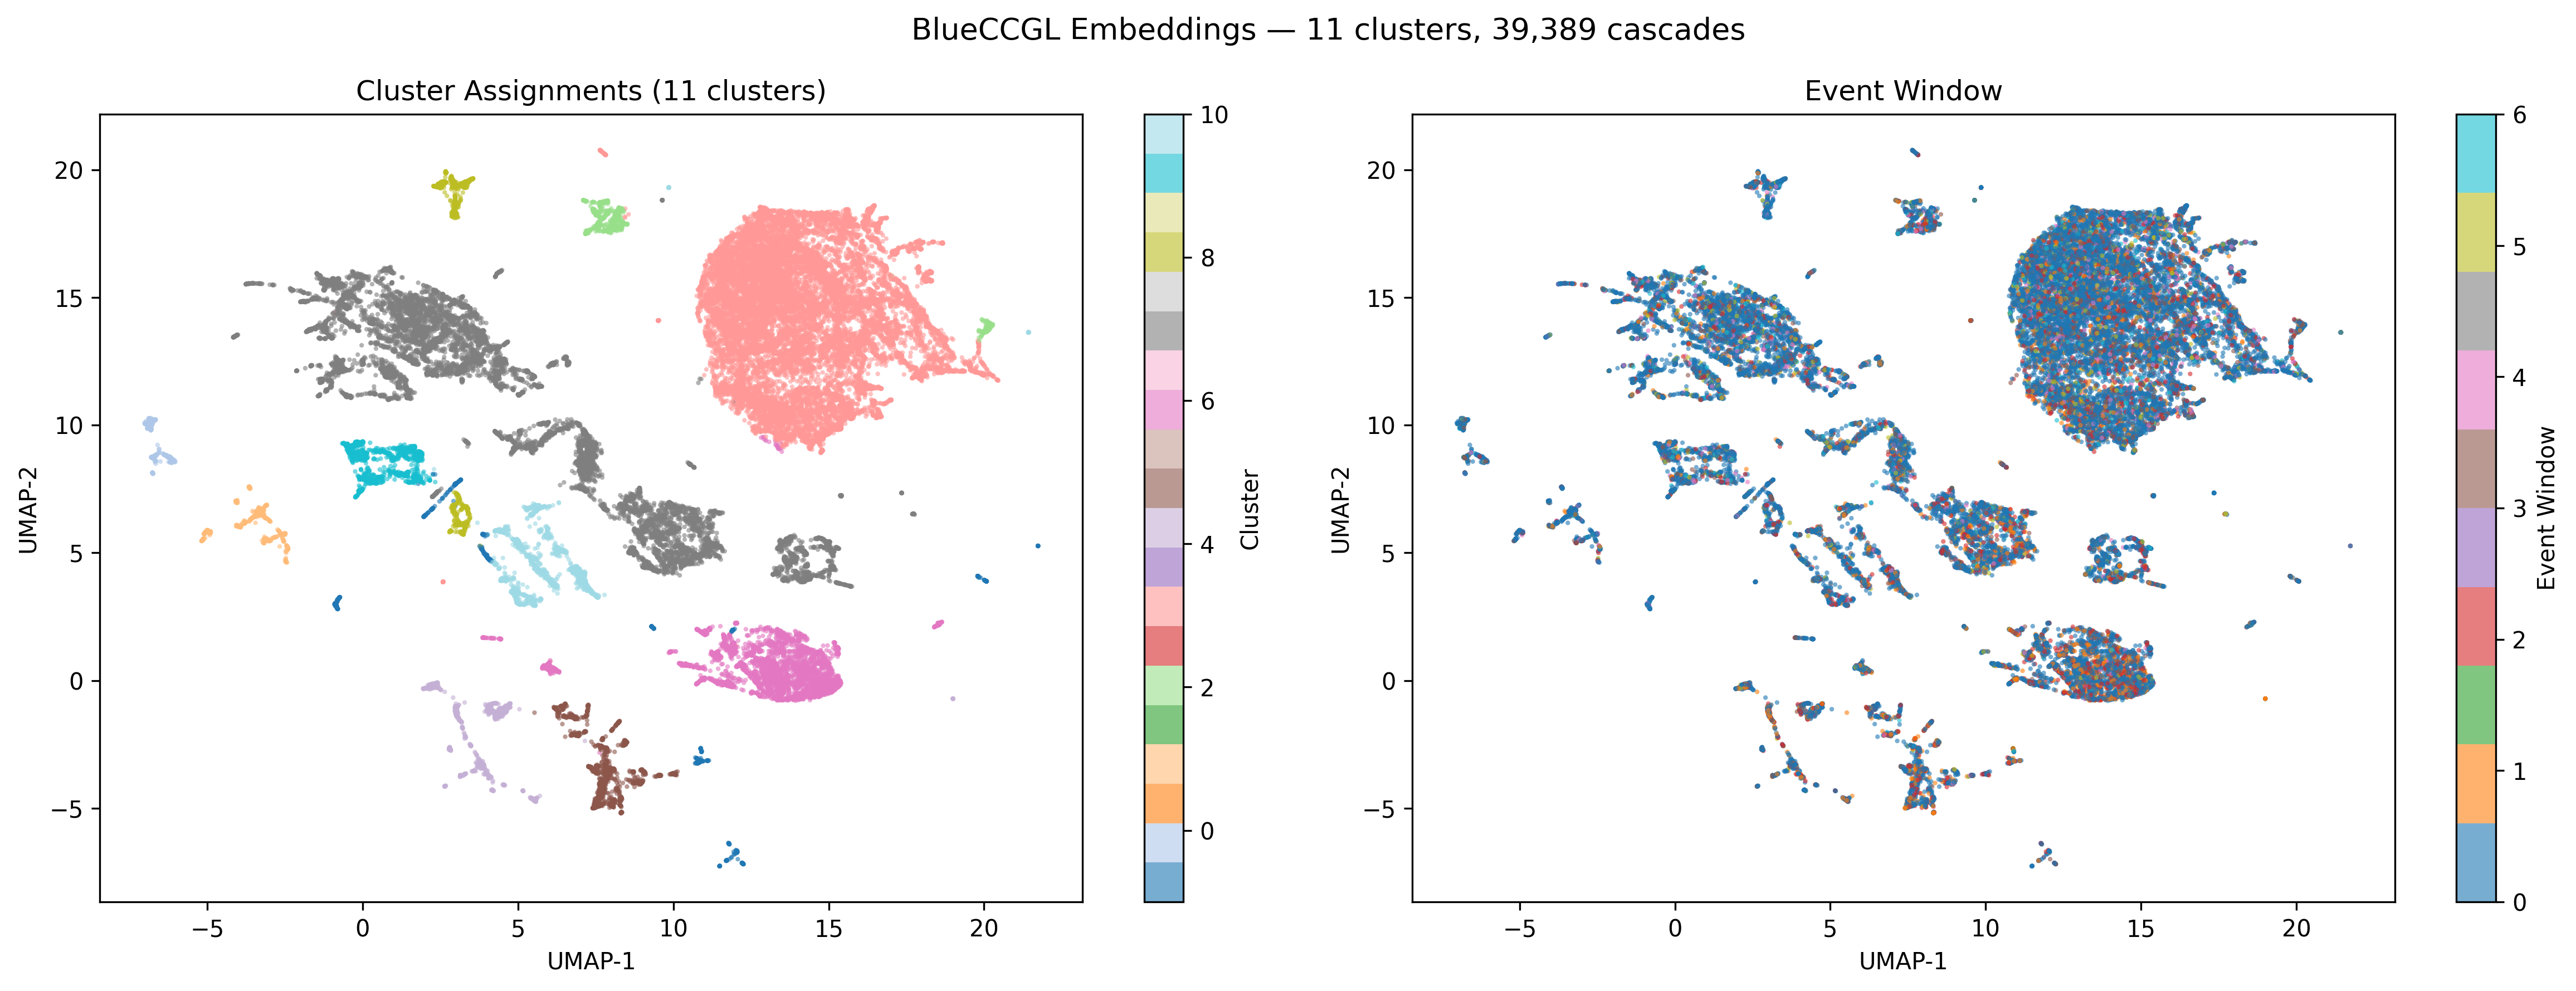
\includegraphics[width=\textwidth]{umap_figure.png}
\caption{UMAP two-dimensional projection of all 39,983 cascade embeddings. Panel~A: coloured by HDBSCAN cluster label (C0--C10). Panel~B: coloured by event window (E1--E6 and baseline). The clear cluster separation in Panel~A and the absence of event-window clustering in Panel~B confirm that the model learned structural rather than temporal signal.}
\label{fig:umap}
\end{figure}

\subsection{Discovered Archetypes}
\label{sec:archetypes}

\BLUECCGL identified 11 cascade archetypes, summarised in Table~\ref{tab:archetypes}. For interpretability these are grouped into six structural families based on shared sentinel properties.

\begin{table}[H]
\centering
\caption{Cluster structural profiles --- all 11 archetypes.}
\label{tab:archetypes}
\small
\begin{tabular}{@{}lrrlllll@{}}
\toprule
\textbf{Cluster} & \textbf{n} & \textbf{\%} & \textbf{Depth med} & \textbf{Breadth med} & \textbf{Size med} & \textbf{Follower ratio} & \textbf{Sentiment} \\
\midrule
C0  & 355    & 0.9\%  & 4   & 2 & 6  & 0.62          & 100\% negative \\
C1  & 670    & 1.7\%  & 3   & 4 & 7  & 0.84          & 100\% negative \\
C2  & 785    & 2.0\%  & 3   & 4 & 7  & 0.76          & 82\% neg / 18\% pos \\
C3  & 16,834 & 42.1\% & 5   & 6 & 16 & 0.78          & 59\% neg / 28\% neu / 13\% pos \\
C4  & 1,020  & 2.6\%  & 4   & 3 & 7  & 0.75          & 100\% neutral \\
C5  & 1,489  & 3.7\%  & 3.5 & 4 & 9  & 0.91          & 100\% neutral \\
C6  & 3,554  & 8.9\%  & 4   & 6 & 13 & 0.85          & 90\% neutral \\
C7  & 11,009 & 27.5\% & 3   & 4 & 9  & 0.82          & 65\% neg / 35\% neu \\
C8  & 833    & 2.1\%  & 5   & 2 & 8  & \textbf{0.51} & 78\% negative \\
C9  & 1,222  & 3.1\%  & 4.5 & 3 & 8  & 0.69          & 80\% negative \\
C10 & 1,618  & 4.0\%  & 4.5 & 3 & 7  & 0.66          & 50\% neg / 50\% neu \\
\bottomrule
\end{tabular}
\end{table}

\begin{figure}[H]
\centering
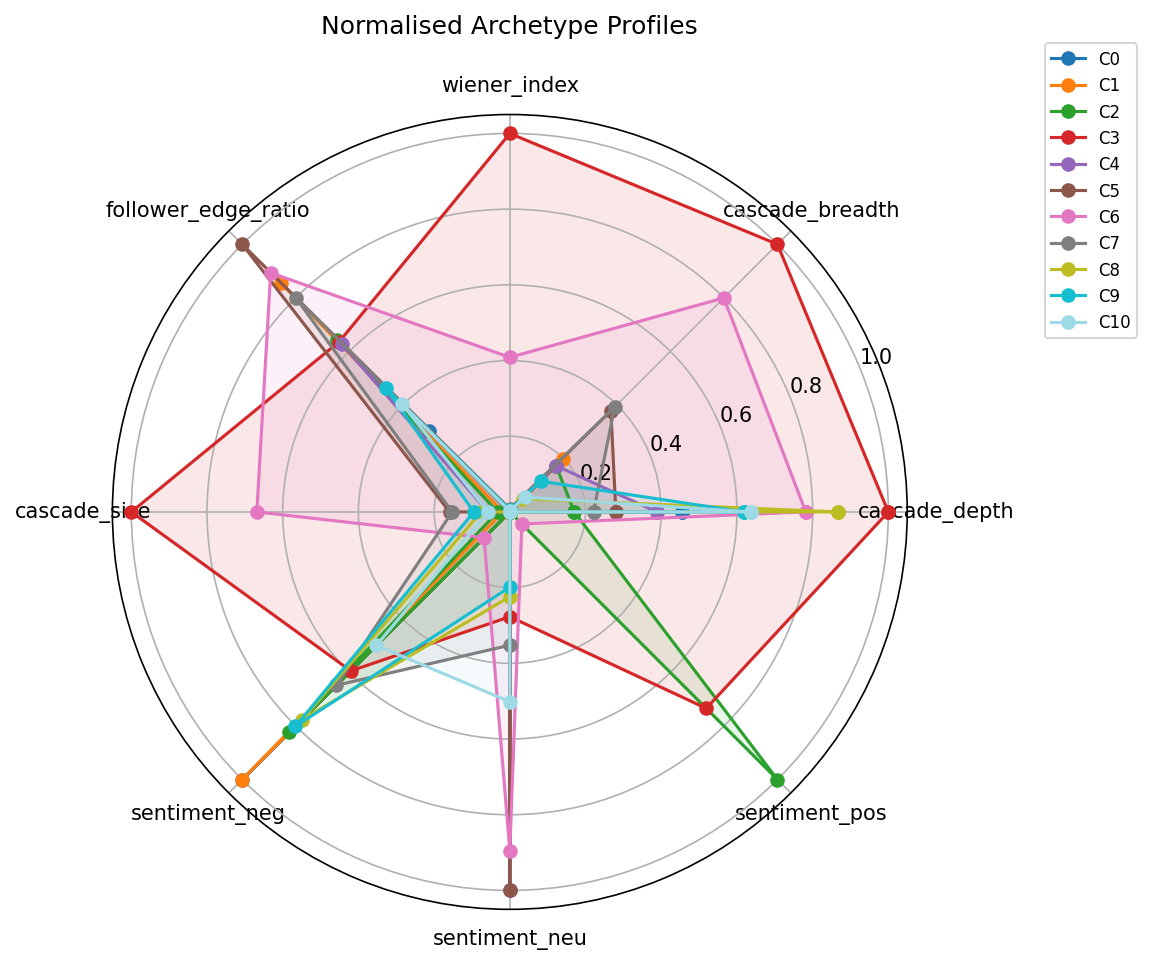
\includegraphics[width=0.9\textwidth]{cluster_radar_profiles.png}
\caption{Normalised structural profiles for all 11 clusters displayed as a radar chart. C8 is visually distinct on the follower-ratio axis (lowest at 0.51), C5 is distinct on the opposite end (highest at 0.91), and C3 projects strongly on the size and breadth axes.}
\label{fig:radar}
\end{figure}

\subsubsection*{Family~1 --- Pure Negative Reaction Cascades (C0, C1)}

C0 ($n\!=\!355$) and C1 ($n\!=\!670$) both exhibit \textbf{100\% negative sentiment} with zero standard deviation --- every post in every cascade in these two clusters carries a negative sentiment label from the pre-computed RoBERTa annotation. Despite this shared sentiment property, they are structurally distinct. C0 is deep-narrow (depth\,=\,4, breadth\,=\,2, follower ratio\,=\,0.62): these are sustained back-and-forth negative exchanges that drew meaningful non-follower engagement. C1 is shallow-wide (depth\,=\,3, breadth\,=\,4, follower ratio\,=\,0.84): a root post that triggered immediate negative responses from many followers simultaneously.

\textbf{Interpretation.} C0 likely represents sustained negative debate threads --- posts about acute traumatic events that drew both community members and outside voices into extended negative argument. C1 represents negative community consensus cascades --- a post that catalysed immediate, broad disapproval within the poster's follower network without drawing sustained outside engagement.

\subsubsection*{Family~2 --- Near-Negative Mixed Cascades (C2)}

C2 ($n\!=\!785$) is structurally similar to C1 (depth\,=\,3, breadth\,=\,4, follower ratio\,=\,0.76) but its sentiment composition departs from uniformity: 82\% negative, 18\% positive. The 18\% positive admixture distinguishes these from the pure-negative clusters; these are predominantly negative threads that contain a visible minority of positive responses --- likely solidarity posts, expressions of hope, or counter-voices within an otherwise distressed discussion.

\textbf{Interpretation.} C2 represents the typical mixed reaction thread where grief or outrage is dominant but some hope or solidarity is visible --- the characteristic discourse pattern of communities processing a traumatic event that admits of both emotional response and community cohesion.

\subsubsection*{Family~3 --- Dominant Discussion Mode (C3)}

C3 ($n\!=\!16{,}834$, 42.1\% of all cascades) is the largest cluster by a substantial margin. It represents the characteristic mode of crisis communication on Bluesky: substantive multi-level discussion threads reaching 5 reply levels deep, branching into 6+ sub-threads at the median, with a median cascade size of 16 posts and a long right tail extending to hundreds of nodes. The sentiment composition (59\% negative, 28\% neutral, 13\% positive) reflects genuine ongoing discussion rather than uniform emotional reaction. The 78\% follower ratio indicates that most engagement comes from within the poster's network, but 22\% of interactions cross community boundaries.

\textbf{Interpretation.} C3 is the workhorse of conflict discourse on Bluesky: the community's preferred mode for processing, discussing, and elaborating on crisis events. The large size, moderate depth, and cross-community reach suggest these are posts that matter enough to generate sustained engagement but are not so extreme as to drive exclusively outside (algorithmic) traffic.

\subsubsection*{Family~4 --- Pure Informational Community Posts (C4, C5)}

C4 ($n\!=\!1{,}020$) and C5 ($n\!=\!1{,}489$) both exhibit \textbf{100\% neutral sentiment} with zero variance. They differ primarily in follower ratio: C5 has a follower ratio of 0.91 --- the highest in the dataset --- indicating that nearly all interactions are between mutual followers. C4 has a moderate follower ratio of 0.75.

\textbf{Interpretation.} C4 and C5 represent purely informational posts --- news updates, factual sharing, resource links, or community announcements --- that generated structured engagement. C5 in particular, with its near-maximal follower ratio and entirely neutral sentiment, represents insular community coordination: information circulated within a closed community of mutual followers, consistent with logistical or organisational posts during crisis periods.

\subsubsection*{Family~5 --- Medium Neutral-to-Negative Threads (C6, C7)}

C6 ($n\!=\!3{,}554$, 8.9\%) and C7 ($n\!=\!11{,}009$, 27.5\%) together account for 36\% of all cascades. C6 is predominantly neutral (90\%), larger (median size\,=\,13), and broader (breadth\,=\,6) with a high follower ratio (0.85). C7 is majority-negative (65\%), smaller (median size\,=\,9), and still primarily follower-driven (0.82).

\textbf{Interpretation.} C6 represents medium-sized neutral discussion threads that grew into multi-level engagement. C7 represents the workhorse of negative conflict commentary at the medium scale. Together C3, C6, and C7 account for 79\% of all cascades, forming the core of how this community processed the conflict.

\subsubsection*{Family~6 --- Cross-Community Debate (C8)}

C8 ($n\!=\!833$, 2.1\%) is the structurally most distinctive cluster in the dataset. Its \textbf{follower edge ratio of 0.51} is the lowest of any cluster: half of all cascade edges in C8 connect users who do not follow each other, indicating that these cascades crossed community boundaries to an extent not seen elsewhere. Combined with a deep-narrow shape (depth\,=\,5, breadth\,=\,2) and 78\% negative sentiment, these are sustained back-and-forth exchanges between people who do not follow each other --- cross-community arguments or debates, likely triggered by contentious posts that provoked extended engagement from outside the poster's network.

\textbf{Interpretation.} C8 represents algorithmically-amplified or cross-community debate threads --- the crisis cascade archetype most strongly associated with non-organic spread. The augmentation sensitivity analysis (Section~\ref{sec:augsens}) confirms that C8 embeddings are the most sensitive to bridge-node removal in the dataset (sensitivity\,=\,1.22), directly validating that these cascades are structurally defined by their non-follower entry points.

\subsubsection*{Family~7 --- Moderate Cross-Community Chains (C9, C10)}

C9 ($n\!=\!1{,}222$) and C10 ($n\!=\!1{,}618$) share a deep-narrow shape (depth\,$\approx$\,4.5, breadth\,$\approx$\,3) and moderate cross-community spread (follower ratio 0.66--0.69). They differ in sentiment: C9 is strongly negative (80\%) while C10 splits evenly between negative and neutral (50/50). Both show elevated bridge-removal sensitivity (C9\,=\,0.84, C10\,=\,0.86), confirming that their moderate non-follower component plays a structurally meaningful role.

\textbf{Interpretation.} C9 and C10 represent moderate cross-community debate chains --- threads that drew partial outside engagement without reaching the extreme cross-community exposure of C8.

\subsection{What the Model Learned --- Linear Probing}
\label{sec:probing}

Linear probes test whether a linear model can decode structural properties from the frozen 64-dimensional embeddings. $R^2 > 0$ indicates the property is linearly encoded (Table~\ref{tab:probes}).

\begin{table}[H]
\centering
\caption{Linear probe results on frozen 64D embeddings.}
\label{tab:probes}
\small
\begin{tabularx}{\textwidth}{@{}lllrX@{}}
\toprule
\textbf{Property} & \textbf{Probe} & \textbf{Global score} & \textbf{95\% CI} & \textbf{Within-cluster range} \\
\midrule
Follower edge ratio & Ridge $R^2$          & \textbf{0.941}   & [0.949, 0.952] & 0.917--0.981 \\
Cascade depth       & Ridge $R^2$          & \textbf{0.686}   & [0.807, 0.823] & 0.697--0.824 \\
Cascade breadth     & Ridge $R^2$          & 0.317            & [0.742, 0.773] & 0.333--0.938 \\
Cascade size        & Ridge $R^2$          & $-6.07$ (global) & [0.495, 0.544] & 0.686--0.911 (within-cluster) \\
Wiener index        & Ridge $R^2$          & $-31{,}876$      & [$-0.012$, 0.147] & Not meaningful \\
Event window        & LogReg bal.\ acc.   & \textbf{0.143}   & [0.143, 0.143] & 0.142--0.148 \\
\bottomrule
\end{tabularx}
\end{table}

\begin{figure}[H]
\centering
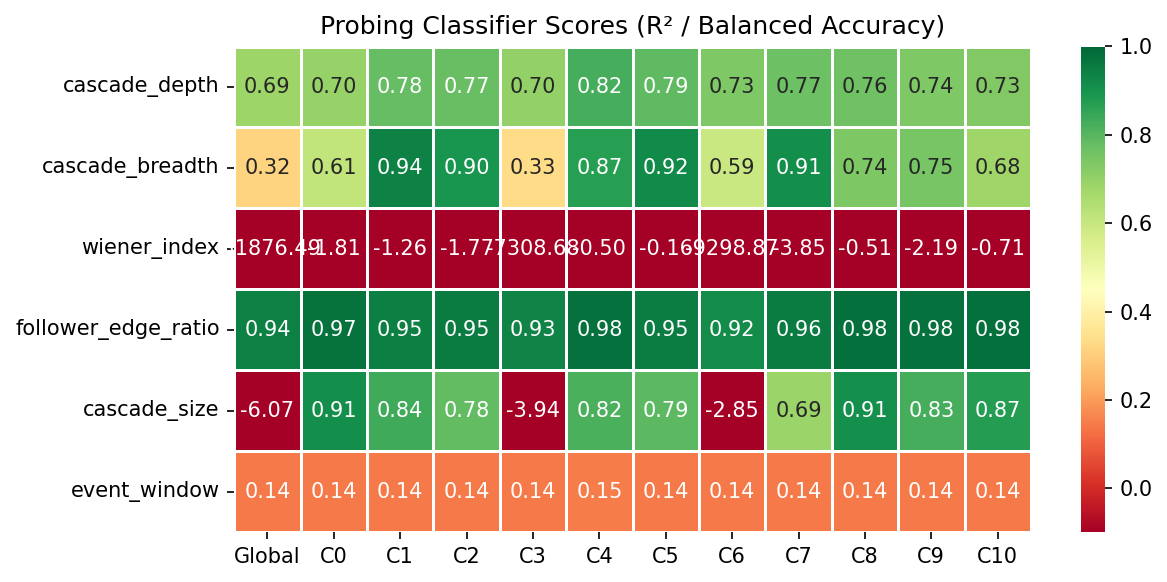
\includegraphics[width=0.95\textwidth]{probe_heatmap.png}
\caption{Linear probe $R^2$ (regression) or balanced accuracy (classification) per property (rows) and cluster (columns). Follower edge ratio dominates as the most linearly encoded property across all 11 clusters ($R^2 = 0.917$--$0.981$). Event window balanced accuracy equals chance ($1/7 \approx 0.143$) universally.}
\label{fig:probes}
\end{figure}

The follower edge ratio probe result ($R^2 = 0.941$ globally, consistent 0.917--0.981 within every cluster) is the dominant finding of the probing analysis. The contrastive model has learned to encode almost perfectly whether a cascade propagated through organic follower-based channels versus non-follower cross-community channels. This is a direct consequence of Extension~2 (R-GCN edge-type encoding).

Cascade depth ($R^2 = 0.686$) is the second strongest encoded property. Cascade breadth shows an interesting dissociation: the global $R^2$ is moderate (0.317) because breadth varies substantially \textit{between} clusters, but within-cluster $R^2$ is high (0.333--0.938), particularly in clusters with uniform breadth distributions (C1\,=\,0.938, C5\,=\,0.920, C7\,=\,0.914).

Cascade size shows a global $R^2$ of $-6.07$ --- a failure of global linear decoding driven by clusters C3 and C6, which absorb the majority of cascades with high internal variance in cascade size. Within each cluster, size is well-encoded ($R^2 = 0.686$--$0.911$).

The event window probe at exactly 0.143 balanced accuracy --- equal to the $1/7$ chance level --- is definitive: the embeddings carry \textit{no} temporal information whatsoever. The model learned the \textit{structure} of how information cascaded, not \textit{when} it did so.

\subsection{Augmentation Sensitivity Analysis}
\label{sec:augsens}

For each cluster, 20 representative cascades were subjected to each of the three feed-aware augmentation strategies. Table~\ref{tab:augsens} reports the mean cosine distance between original and augmented embeddings.

\begin{table}[H]
\centering
\caption{Augmentation sensitivity (mean cosine distance, range 0--2) per cluster.}
\label{tab:augsens}
\small
\begin{tabular}{@{}lrrrL{4cm}@{}}
\toprule
\textbf{Cluster} & \textbf{Follower sub. (A)} & \textbf{Temp. prefix (B)} & \textbf{Bridge rem. (C)} & \textbf{Primary driver} \\
\midrule
C0  & N/A\textsuperscript{\dag} & 0.944 & 0.545 & Temporal ordering \\
C1  & 0.998 & 0.820 & 0.539 & Follower structure + timing \\
\textbf{C2}  & \textbf{1.979} & 0.889 & 0.474 & Strongly follower-edge dependent \\
C3  & 1.074 & 0.938 & 0.686 & All signals; heterogeneous cluster \\
C4  & N/A\textsuperscript{\dag} & 0.922 & 0.671 & Temporal ordering \\
C5  & 0.948 & \textbf{1.193} & 0.446 & Early temporal prefix carries structure \\
C6  & 1.067 & 0.996 & 0.785 & Balanced across all augmentations \\
C7  & 1.253 & 0.942 & 0.691 & Follower structure primary \\
\textbf{C8}  & N/A\textsuperscript{\dag} & \textbf{1.308} & \textbf{1.220} & Uniquely sensitive to bridge removal \\
C9  & 1.004 & \textbf{1.148} & 0.835 & Temporal + bridge signals \\
C10 & N/A\textsuperscript{\dag} & 0.930 & 0.856 & Bridge removal informative \\
\bottomrule
\multicolumn{5}{@{}l}{\textsuperscript{\dag} Insufficient follower edges to survive the 30\% retention ratio augmentation.}
\end{tabular}
\end{table}

\begin{figure}[H]
\centering
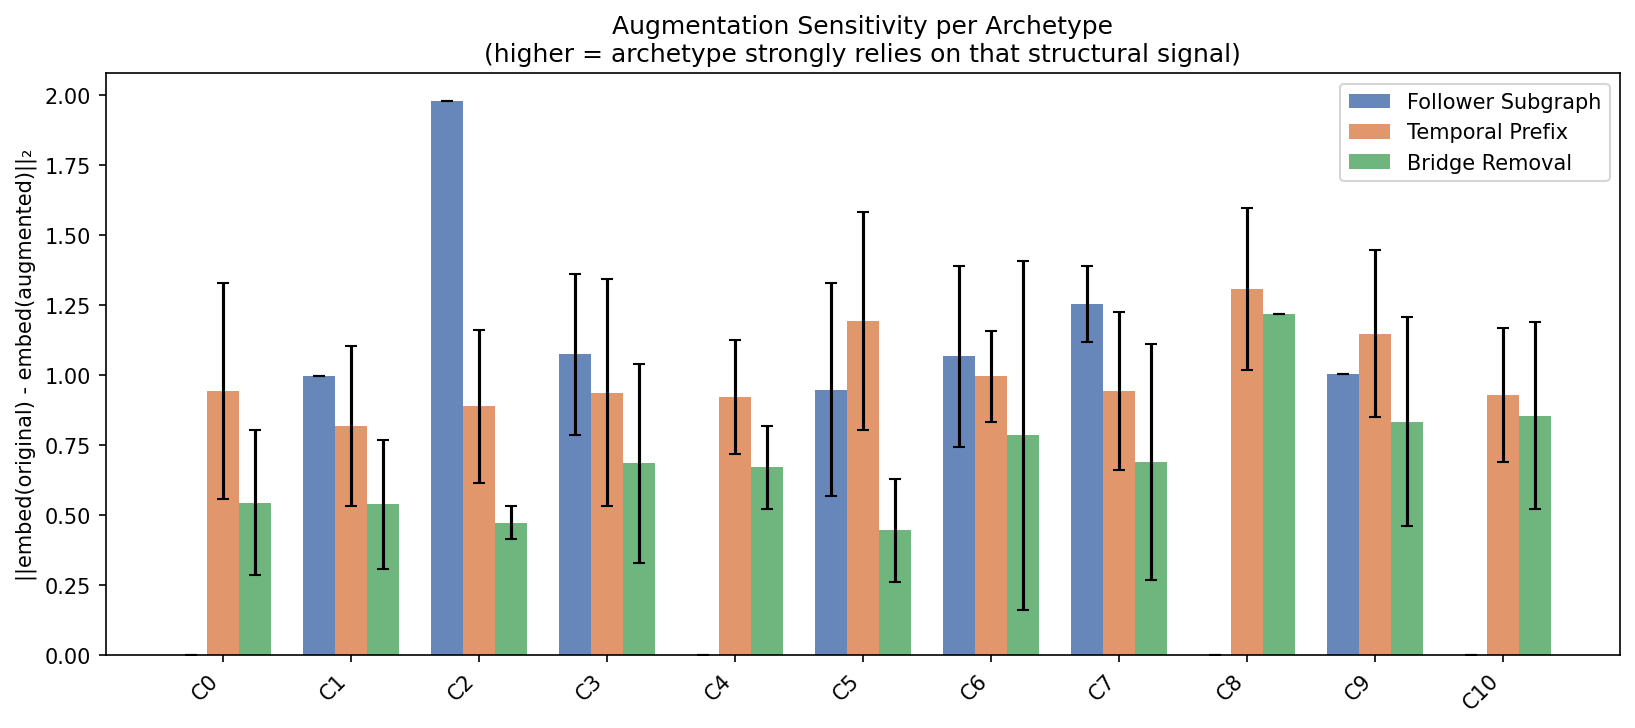
\includegraphics[width=\textwidth]{augmentation_sensitivity_bars.png}
\caption{Augmentation sensitivity grouped bar chart per cluster. Each bar group shows the mean cosine distance under each of the three augmentation strategies. C8's uniquely high bridge-removal sensitivity (1.22) confirms that cross-community debate cascades are structurally defined by their non-follower entry points.}
\label{fig:augsens}
\end{figure}

The C8 bridge-removal sensitivity of 1.22 is the highest in the dataset and represents a direct structural validation of the cross-community debate interpretation. C2's follower-subgraph sensitivity of 1.979 --- approaching the maximum possible cosine distance of 2.0 --- indicates that the near-negative mixed cascades are almost entirely dependent on their follower-edge topology. C5's elevated temporal prefix sensitivity (1.193) suggests that the early portion of insular community coordination cascades carries disproportionate structural information.

\subsection{Archetype Composition Across Mega-Events}

Table~\ref{tab:eventtab} presents the archetype $\times$ event-window cross-tabulation: the percentage of each event window's cascades assigned to each cluster. The event window probe (balanced accuracy\,=\,0.143) confirmed that the embeddings do not linearly encode event-window membership; archetype composition differences therefore reflect genuine structural differences in how different crisis event types generate different cascade shapes.

\begin{table}[H]
\centering
\caption{Archetype composition per event window (\% of cascades in each window).}
\label{tab:eventtab}
\footnotesize
\begin{tabular}{@{}lrrrrrrrrrrrr@{}}
\toprule
\textbf{Event} & \textbf{n} & \textbf{C0} & \textbf{C1} & \textbf{C2} & \textbf{C3} & \textbf{C4} & \textbf{C5} & \textbf{C6} & \textbf{C7} & \textbf{C8} & \textbf{C9} & \textbf{C10} \\
\midrule
Baseline        & 27,163 & 1.0 & 1.8 & 1.9 & 43.2 & 2.4 & 3.3 & 8.0  & 28.7 & 2.3 & 3.2 & 4.2 \\
E1 (Oct 7)      & 2,686  & 0.5 & 1.2 & 1.6 & 33.4 & \textbf{5.1} & \textbf{9.1} & \textbf{19.7} & 23.3 & 0.8 & 1.6 & 3.6 \\
E2 (Al-Ahli)    & 3,285  & 0.3 & 1.0 & 2.1 & 39.6 & 4.0 & 6.8 & \textbf{15.9} & 23.4 & 1.2 & 2.3 & 3.5 \\
E3 (Ceasefire)  & 2,671  & 0.9 & 1.9 & 1.9 & \textbf{46.7} & 2.6 & 3.0 & 7.7 & 26.4 & 1.9 & 3.2 & 3.8 \\
E4 (ICJ)        & 1,304  & 1.0 & 2.9 & 3.0 & \textbf{48.1} & 1.0 & 0.9 & 3.5 & 28.9 & 2.5 & 3.5 & 4.7 \\
E5 (Bushnell)   & 1,364  & 0.8 & 1.6 & 2.4 & 44.6 & 0.9 & 1.1 & 4.1 & \textbf{32.7} & 2.2 & 4.3 & \textbf{5.3} \\
E6 (Flour)      & 916    & 0.5 & 1.2 & 2.5 & 47.2 & 0.4 & 1.5 & 3.3 & \textbf{31.3} & \textbf{3.3} & 4.1 & \textbf{4.6} \\
\bottomrule
\multicolumn{13}{@{}l}{\textit{Bold values indicate notable deviations from the baseline distribution.}}
\end{tabular}
\end{table}

\begin{figure}[H]
\centering
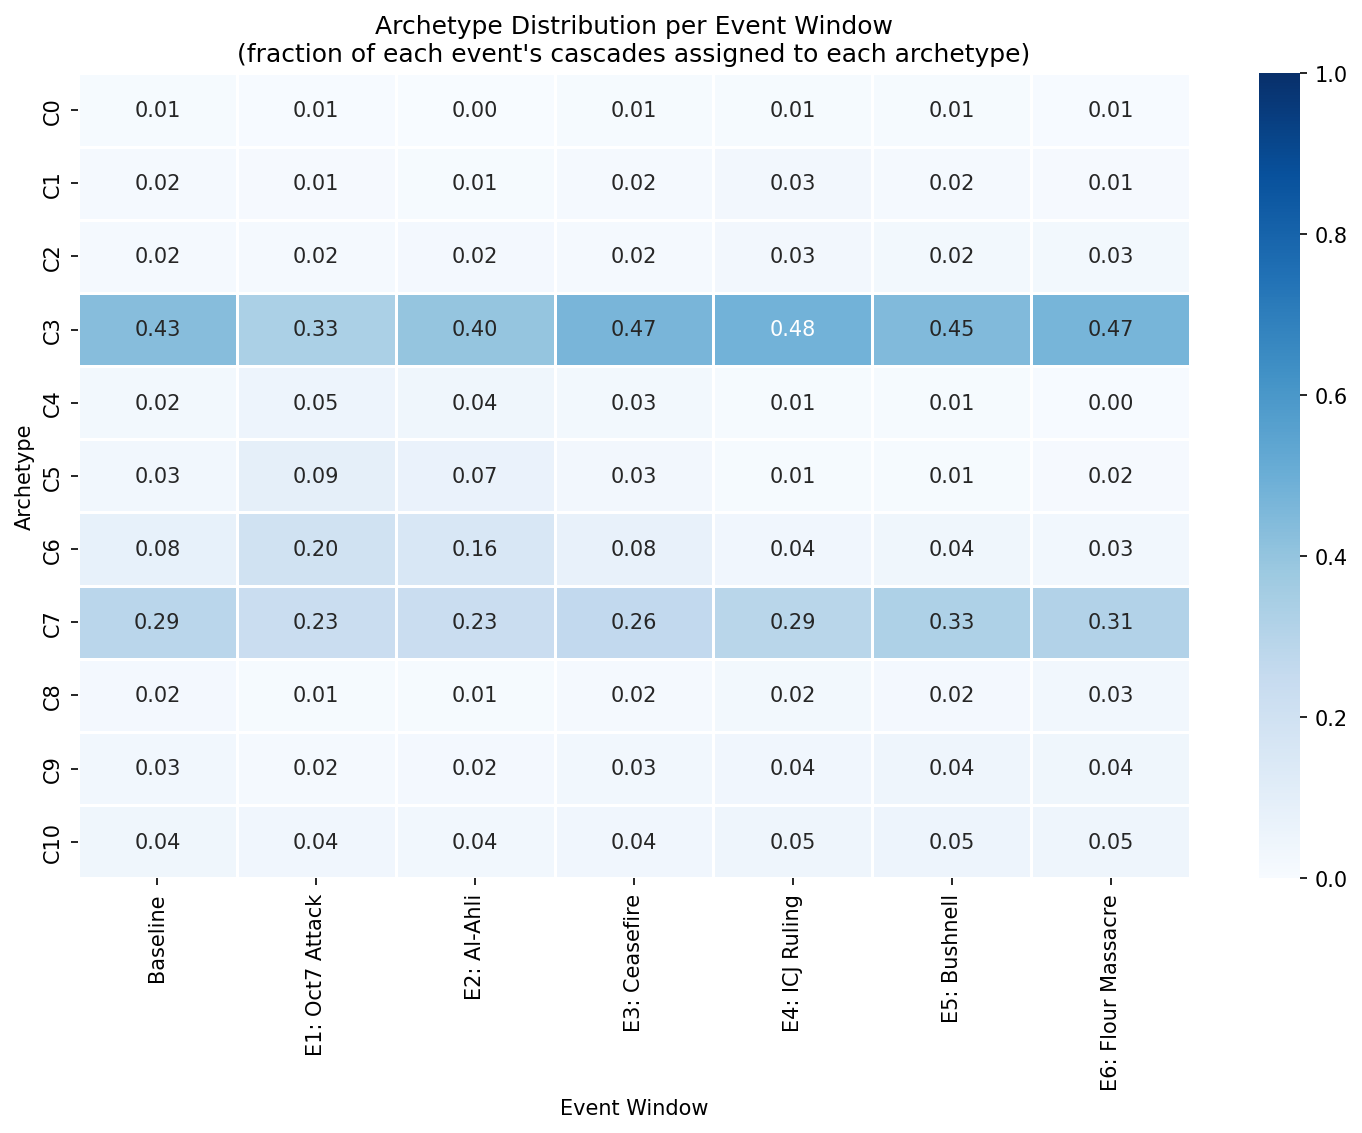
\includegraphics[width=\textwidth]{archetype_event_heatmap.png}
\caption{Archetype $\times$ event-window fraction heatmap. Columns represent event windows; rows represent clusters. Deviations from the baseline column indicate event-specific archetype surges.}
\label{fig:eventheatmap}
\end{figure}

\begin{figure}[H]
\centering
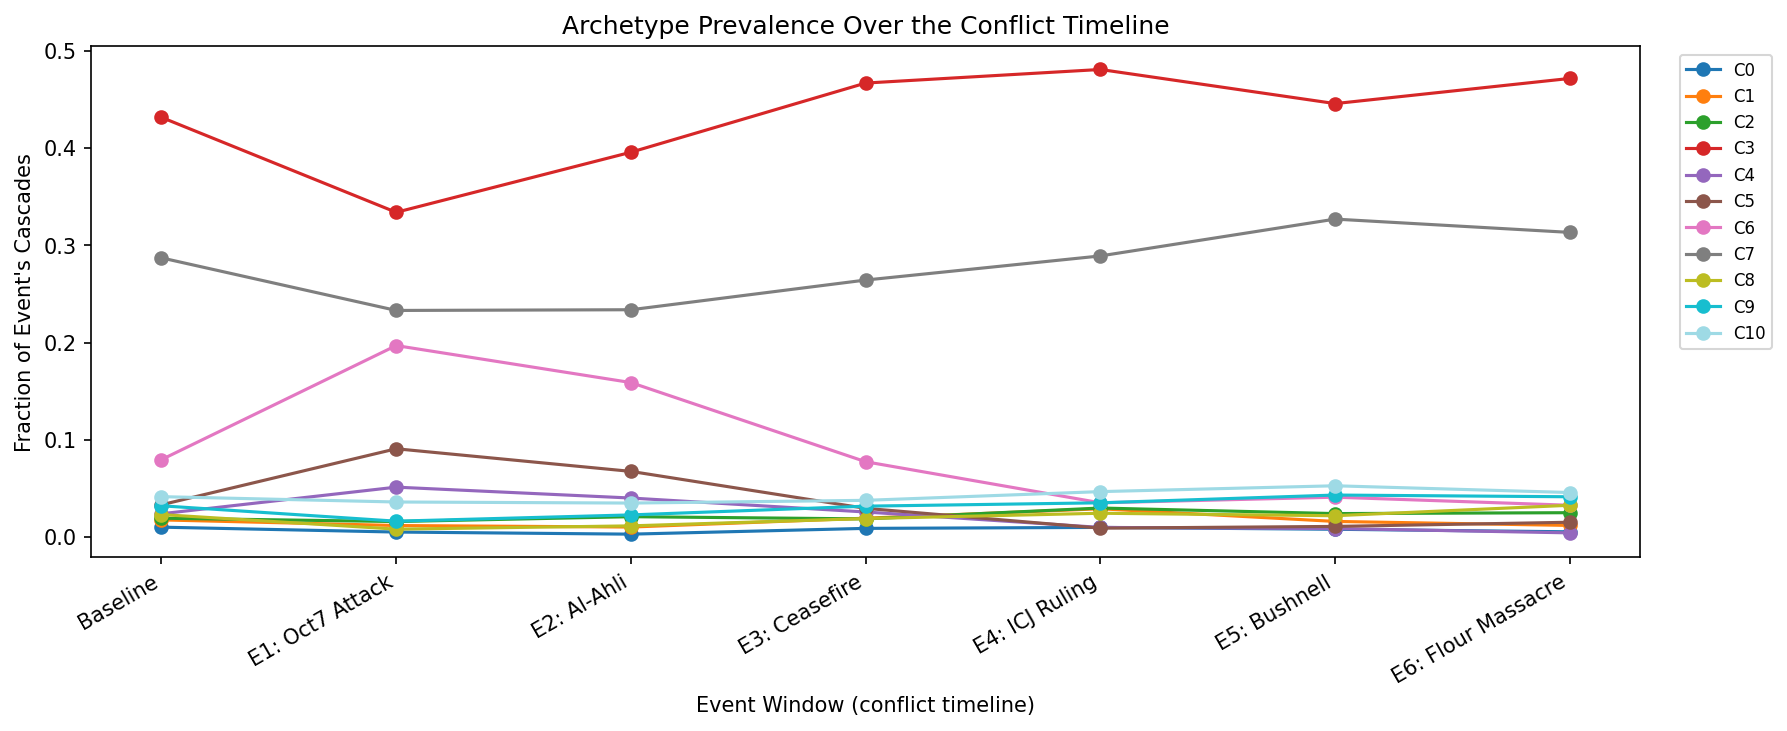
\includegraphics[width=\textwidth]{temporal_evolution.png}
\caption{Temporal evolution of archetype prevalence fractions across the conflict timeline (E1--E6 and baseline). Lines represent individual cluster fractions over time.}
\label{fig:temporal}
\end{figure}

\begin{figure}[H]
\centering
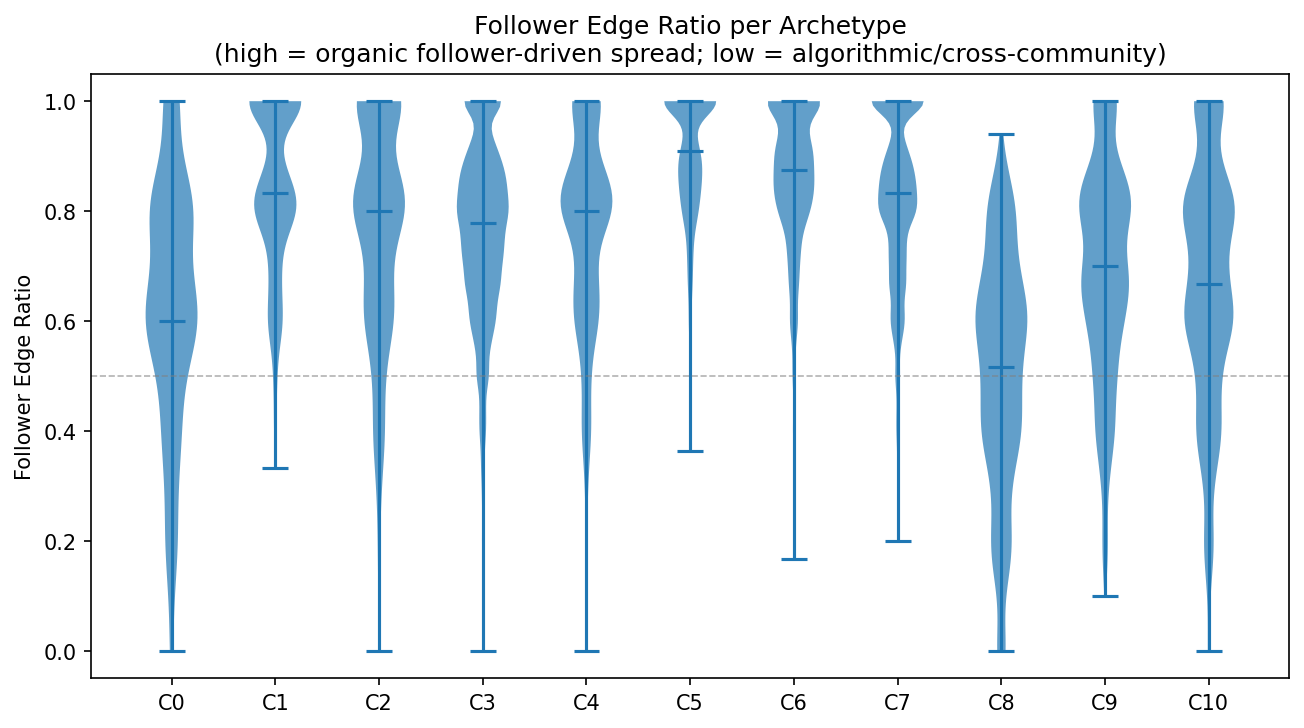
\includegraphics[width=0.9\textwidth]{follower_ratio_violins.png}
\caption{Distribution of follower edge ratio per cluster displayed as violin plots. C8 (cross-community debate) is clearly separated at the low end (centred at 0.51); C5 (insular community coordination) is separated at the high end (centred at 0.91).}
\label{fig:violins}
\end{figure}

\subsection{Research Question Answers}

\subsubsection*{SRQ1: Crisis Phase Evolution}

\textbf{Partial yes, with caveats.} The archetype $\times$ event-window cross-tabulation reveals systematic shifts in archetype composition that are not attributable to embedding-level temporal encoding.

The most striking pattern is the E1 surge in neutral informational archetypes: C5 (insular community coordination) rises from 3.3\% at baseline to 9.1\% during E1, and C6 (medium neutral discussion) rises from 8.0\% to 19.7\%. This is consistent with the breaking-news dynamics of October~7: in the immediate aftermath of an acute shock event, users circulate factual information and updates before the emotional/deliberative phase begins. The C3 large discussion cluster, by contrast, \textit{drops} from 43.2\% at baseline to 33.4\% during E1 --- the dominant deliberative mode is temporarily displaced by informational cascades during acute shock. By E4 (ICJ ruling), C3 peaks at 48.1\% and the informational archetypes reach their lowest values, consistent with the expected temporal narrative: as the conflict matures from acute shock to sustained advocacy, discourse shifts from broadcasting updates to sustained deliberative engagement.

\textbf{Caveat.} The differences are modest (a few percentage points in most cases) and the dominant pattern is stability of archetype composition across events, with C3 dominating (33--48\%) throughout.

\subsubsection*{SRQ2: Event-Type Structural Signatures}

\textbf{Yes, with interpretable patterns.}
\begin{itemize}
  \item \textbf{Acute military shock (E1):} Highest informational archetype share (C5\,=\,9.1\%, C6\,=\,19.7\%), lowest C3 (33.4\%). Breaking-news dynamics dominate.
  \item \textbf{Contested humanitarian event (E2, Al-Ahli):} Intermediate; C6 remains elevated (15.9\%). Contested attribution may prolong the informational phase.
  \item \textbf{Diplomatic multi-day event (E3, ceasefire):} Highest C3 share (46.7\%) among the first four events. The sustained character generates large deliberative discussions.
  \item \textbf{Legal/institutional milestone (E4, ICJ):} Highest overall C3 share (48.1\%), lowest informational archetypes. Legal milestones generate the most deliberative, sustained discussion.
  \item \textbf{Individual human story (E5, Bushnell):} Highest C7 share (32.7\%). Individual emotionally resonant events generate sustained negative mid-scale engagement.
  \item \textbf{Compound humanitarian/milestone (E6, flour massacre):} Highest C8 share (3.3\%). Cross-community debate peaks during humanitarian milestone events.
\end{itemize}

\subsubsection*{SRQ3: Algorithmic Amplification}

\textbf{Predominantly organic, but with a distinct minority cross-community archetype.} At the dataset level, 75.9\% of all cascade edges are FOLLOWER-typed. The vast majority of crisis information spread was organic. Non-follower edges account for 24.1\%, representing cross-community or algorithmically-exposed spread. The follower edge ratio probe ($R^2 = 0.941$) confirms this is the primary structural axis encoded in \BLUECCGL embeddings. Only 2.1\% of cascades are in C8 (the primary cross-community debate archetype), but C8 is most prevalent during E6 (3.3\%) --- the event with the highest moral salience --- consistent with the hypothesis that content with strong moral framing crosses community boundaries more readily.

\textbf{Caveat.} The temporal confound in the follower graph (Section~\ref{sec:cascade}) means that some FOLLOWER edges for early cascades may not have existed at cascade time. The true non-follower fraction for E1/E2 may be slightly higher than reported.

\subsubsection*{SRQ4: Sentiment-Structure Coupling}

\textbf{Yes, strongly.} Sentiment composition is one of the primary axes along which the learned representation organises cascade archetypes. Four of the eleven clusters are defined by a single dominant sentiment class with zero variance: C0 and C1 (100\% negative), C4 and C5 (100\% neutral). The Kruskal-Wallis $H$-statistic for positive sentiment proportion (34,280) is the highest of any property tested. Crucially, C8 (cross-community debate, follower ratio\,=\,0.51) is predominantly negative (78\%). This coupling --- negative content crossing community boundaries --- is consistent with \citet{vosoughi2018spread}, who found that emotionally negative content spreads faster and deeper than neutral content. On Bluesky, the cascade archetype with the most cross-community spread is also predominantly negative.

\subsubsection*{MRQ1: What natural archetypes emerge?}

\BLUECCGL with HDBSCAN discovers 11 archetypes grouping into six interpretable families: pure negative reaction (C0, C1), near-negative mixed (C2), dominant discussion mode (C3), pure informational community posts (C4, C5), medium neutral-to-negative threads (C6, C7), cross-community debate (C8), and moderate cross-community chains (C9, C10). The primary structural axes are sentiment composition, follower edge ratio, and cascade size/depth. All between-cluster differences are statistically significant at $p < 10^{-300}$.

\subsubsection*{MRQ2: Does R-GCN edge-type encoding improve representation quality?}

The dominant evidence is the follower edge ratio probe result ($R^2 = 0.941$). The R-GCN encoder produces embeddings that encode the organic/algorithmic composition of each cascade almost perfectly. The fact that this signal is present at $R^2 > 0.91$ within every single cluster suggests that edge-type encoding permeates the learned representation uniformly. Ablation study A1 (replacing R-GCN with a homogeneous GCN) will provide the direct quantitative comparison.

\subsubsection*{MRQ3: Do feed-aware augmentations improve representations?}

The augmentation sensitivity analysis provides indirect evidence: the embeddings of different archetype clusters respond differently to the three domain-specific augmentations, with sensitivity patterns that align with the structural interpretations of each archetype. C8's uniquely high bridge-removal sensitivity and C2's near-maximum follower-subgraph sensitivity demonstrate that the feed-aware augmentations capture the structurally defining features of each archetype. Direct ablation comparison (A2: generic augmentation baseline) is planned.

% ============================================================
\section{Next Steps}
\label{sec:nextsteps}

\subsection{Downstream Prediction Tasks}

The pre-trained \BLUECCGL encoder will be evaluated on two downstream transfer tasks (\texttt{--stage downstream}) to assess the quality of learned representations beyond clustering:

\begin{itemize}
  \item \textbf{Cascade size prediction.} A regression head fine-tuned on top of the frozen encoder predicts $\log(\text{cascade\_size})$. Metric: RMSE and $R^2$.
  \item \textbf{Cascade longevity prediction.} A binary classification head predicts whether the cascade remains active beyond the median duration threshold. Metric: AUROC and F1.
\end{itemize}

Baselines: (a) random initialisation (same architecture, no pre-training), (b) vanilla CCGL (generic augmentation, no R-GCN, no DiffPool), (c) handcrafted feature baseline (Wiener index, depth, breadth, branching factor, follower edge ratio fed to a linear MLP). The v8 training results suggest that cascade size will be a challenging target for the frozen encoder (global $R^2 = -6.07$ in the probing experiment), while follower-related structural properties should transfer well ($R^2 = 0.941$).

\subsection{Stability Analysis}

The stability analysis (\texttt{--stage stability}) evaluates the robustness of the discovered 11-archetype solution to perturbations of the cascade dataset:

\begin{itemize}
  \item 10 independent 80\% random subsamples of the 39,983-cascade dataset.
  \item For each subsample: apply HDBSCAN with the selected $\text{min\_cluster\_size} = 300$.
  \item Compute Adjusted Rand Index (ARI) between each pair of subsample cluster assignments.
  \item Report mean $\pm$ std of clustering metrics (Silhouette, DB, CH, DBCV) and ARI across the 10 subsamples.
\end{itemize}

High ARI ($> 0.7$) and low metric variance across subsamples would confirm that the 11-archetype solution is not an artefact of the specific cascade dataset composition.

% ============================================================
\bibliography{references}

\end{document}
